\documentclass[usenames,dvipsnames]{beamer}
\usepackage{tikz}
\usepackage{filecontents}
\usetheme{Madrid}
\usepackage[
    citestyle=numeric,  % Your citation style.
    bibstyle=numeric,         % Style for bibliography list. It will be numeric.
    sorting=none,             % The citations will be listed in the order of appearance
    backend=biber             % This is not necessary for newer versions of biblatex as
                              % it is the default, but it certainly helps to keep things
                              % explicit.
]{biblatex}
%\addbibresource{Bibliography/references}
\setbeamertemplate{bibliography item}{\insertbiblabel}
\addbibresource{\jobname.bib}
\begin{filecontents}{\jobname.bib}

@Article{journals/corr/PengSLMW16,
  title =	"Recent Advances in Cloud Radio Access Networks: System
		 Architectures, Key Techniques, and Open Issues",
  author =	"Mugen Peng and Yaohua Sun and Xuelong Li and Zhendong
		 Mao and Chonggang Wang",
  journal =	"CoRR",
  year = 	"2016",
  volume =	"abs/1604.00607",
  bibdate =	"2017-06-07",
  bibsource =	"DBLP,
		 http://dblp.uni-trier.de/db/journals/corr/corr1604.html#PengSLMW16",
  URL =  	"http://arxiv.org/abs/1604.00607",
}


@Article{journals/twc/TangTQ15,
  title =	"Cross-Layer Resource Allocation With Elastic Service
		 Scaling in Cloud Radio Access Network",
  author =	"Jianhua Tang and Wee-Peng Tay and Tony Q. S. Quek",
  journal =	"IEEE Trans. Wireless Communications",
  year = 	"2015",
  number =	"9",
  volume =	"14",
  bibdate =	"2017-06-09",
  bibsource =	"DBLP,
		 http://dblp.uni-trier.de/https://doi.org/10.1109/TWC.2015.2432023;
		 DBLP,
		 http://dblp.uni-trier.de/db/journals/twc/twc14.html#TangTQ15",
  pages =	"5068--5081",
}


@InProceedings{conf/wiopt/AlabbasiC17,
  title =	"Delay-aware green hybrid CRAN",
  author =	"Abdulrahman Alabbasi and Cicek Cavdar",
  publisher =	"IEEE",
  year = 	"2017",
  bibdate =	"2017-07-06",
  bibsource =	"DBLP,
		 http://dblp.uni-trier.de/https://doi.org/10.23919/WIOPT.2017.7959942;
		 DBLP,
		 http://dblp.uni-trier.de/db/conf/wiopt/wiopt2017.html#AlabbasiC17",
  booktitle =	"WiOpt",
  crossref =	"conf/wiopt/2017",
  ISBN = 	"978-3-9018-8290-6",
  pages =	"1--7",
  URL =  	"http://ieeexplore.ieee.org/xpl/mostRecentIssue.jsp?punumber=7951216",
}
@conference{AnnaV.Guglielmiieee2018,
title = "A baysean Game Theoretic Aproach to Task Offloading in Edge and Cloud Computing",
author = "Anna V. Gugleilmi, Macro Levorato and Leonardo Badia",
publisher = "IEEE"}

@misc{wiki:C-RAN,
   author = "Wikipedia",
   title = "{C-RAN} --- {W}ikipedia{,} The Free Encyclopedia",
   year = "2018",
   howpublished = {\url{http://en.wikipedia.org/w/index.php?title=C-RAN&oldid=827881004}},
   note = "[Online; accessed 26-March-2018]"
 }
 
 

@Article{journals/monet/KhodaRAHAA16,
  title =	"Efficient Computation Offloading Decision in Mobile
		 Cloud Computing over 5G Network",
  author =	"Mahbub E. Khoda and Md. Abdur Razzaque and Ahmad
		 Almogren and Mohammad Mehedi Hassan and Atif Alamri and
		 Abdulhameed Alelaiwi",
  journal =	"MONET",
  year = 	"2016",
  number =	"5",
  volume =	"21",
  bibdate =	"2017-05-20",
  bibsource =	"DBLP,
		 http://dblp.uni-trier.de/https://doi.org/10.1007/s11036-016-0688-6;
		 DBLP,
		 http://dblp.uni-trier.de/db/journals/monet/monet21.html#KhodaRAHAA16",
  pages =	"777--792",
}

 
\end{filecontents}


\logo{%
  \includegraphics[width=1cm,height=1cm,keepaspectratio]{Image/DUlogo.png}%
  \hspace{\dimexpr\paperwidth-2cm-5pt}%
  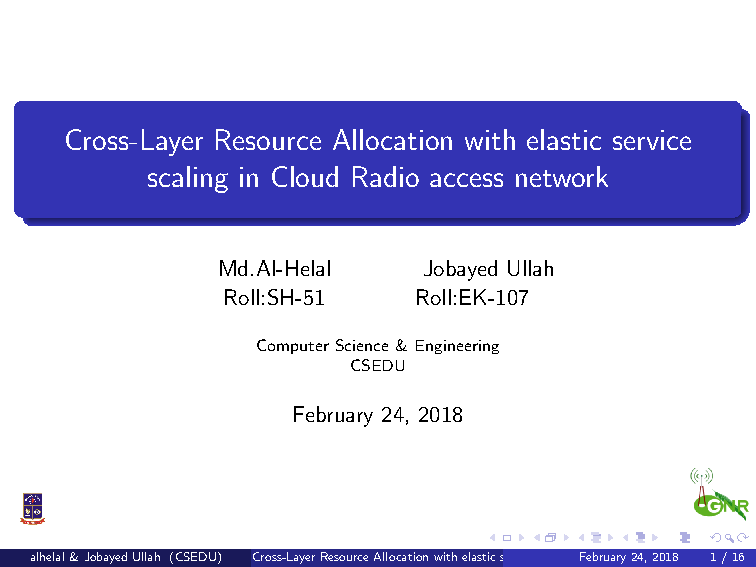
\includegraphics[width=1cm,height=1cm,keepaspectratio]{Image/GNR.jpeg}%
  %\includegraphics[width=1cm,height=1cm,keepaspectratio]{example-image-a}%
}
\begin{document}
  \title{Function Reusing Based Task Distribution between Edge Cloud and Central Cloud in Hybrid CRAN}
  \author[Md.Al-Helal \& Jobayed Ullah]{
  \parbox{2.5cm}{
\centering Md.Al-Helal\\Roll:SH-51}\hspace{3cm}
\parbox{2.5cm}{
{\centering Jobayed Ullah \\Roll:EK-107}}
\centering \vspace{1cm}\\Supervisor:\\Tamal Adhikary\\\scriptsize{Computer Science \& Engineering\\University of Dhaka}
}

\vspace{1cm}
%\institute[CSEDU]{Computer Science \& Engineering\\University of Dhaka}
\date{July 29, 2018}
\begin{frame}
  \maketitle
\end{frame}

\begin{frame}
\frametitle{Contents}
\tableofcontents
\end{frame}
\section{Proposed Model}

\begin{frame}
  \frametitle{Proposed Model}
  \includegraphics[scale=0.25]{Image/edge_cloud_model.png}
\end{frame}

\section{}
\begin{frame}
  \frametitle{Queueing Model}
  \begin{center}
  \includegraphics[scale=0.35]{Image/queue.png}
\end{center}
  \end{frame}

\section{Flowchart}
\begin{frame}
  \frametitle{Flowchart}
  \vspace*{-0.9cm}
  \begin{center}
  \includegraphics[scale=0.3]{Image/flowchart.png}
  \end{center}
  \end{frame}




\section{Proposed Delay Calculation Formula}
\begin{frame}
 \frametitle{Proposed Delay Calculation Formula}
 \begin{equation*}
  \begin{aligned}
   & T_{EC}=t^{EC}_{exe}+t^{EC}_{waiting}+t^{EC}_{VM\ creation}\\
   & T_{CC}=t^{CC}_{exe}+t^{CC}_{trans}\\
  \end{aligned}
 \end{equation*}
 We will calculate $T_{exe}$ using the total number of required CPU cycles to complete a task. And $T_{waiting}$ using the Queueing theory.
\end{frame}

\begin{frame}
  \frametitle{Proposed Delay Calculation Formula}
  \begin{equation}
  \tag{Computation Cost \cite{AnnaV.Guglielmiieee2018}}
   \begin{aligned}
 & K\textsuperscript{EC} = \lambda^tt^{EC}+\lambda^ee^{EC}\\
   & K\textsuperscript{CC} = \lambda^t(t^{CC}_{off}+t^{CC}_{exe})+\lambda^ee^{CC}_{off}\\
 \end{aligned}
 \end{equation}
 Where,  $\lambda^t,\lambda^e \in [0,1]$
 \begin{equation*}
 \tag{Tradeoff Matric \cite{journals/monet/KhodaRAHAA16}}
  \begin{aligned}
   & G = (1- \alpha )\times G_1+\alpha \times G_2\\
  \end{aligned}
 \end{equation*}
 Where, $G_1$ and $G_2$ is gain/loss achieved in time and energy, respectively. $0 \le \alpha \le 1$

\end{frame}

\section{References}
\begin{frame}
  \frametitle{References}
  \printbibliography
%\bibliographystyle{plain} 
\end{frame}

\begin{frame}{\phantom{}}
 % \color{Brown}
  \color{Sepia}
  \centering \Huge\textbf{Thank You}
\end{frame}
\end{document}
